%----------------------------------------------------------------------------------------
%	PACKETS AND CONFIGURATION
%----------------------------------------------------------------------------------------

\documentclass[12pt, a4paper]{article}

\usepackage{times} % Times New Roman font
\usepackage{graphicx} % 'graphics' package interface
\usepackage{geometry} % Edit document margins
\usepackage{hyperref} % Table of contents hyperlinks
\usepackage{tcolorbox} % Colored boxes for code
\usepackage[font=small, labelfont=bf]{caption} % Image caption font

% HELPER PACKAGES (REMOVE IN FINAL) %
\usepackage{blindtext} % Lorem Ipsum
\usepackage{todonotes} % TODOs as useful reminders
\setlength{\marginparwidth}{2cm} % Otherwise todonotes gets angry at me lol
\setuptodonotes{fancyline, color=green!40, shadow} % TODOs options
% HELPER PACKAGES (REMOVE IN FINAL) %

\graphicspath{ {./res/} } % Path to graphics
\hypersetup{    % ToC Hyperlink setup
    colorlinks,
    citecolor=black,
    filecolor=black,
    linkcolor=black,
    urlcolor=black
}

%----------------------------------------------------------------------------------------
%	DOCUMENT
%----------------------------------------------------------------------------------------

\begin{document}

\newgeometry{top=7cm, bottom=2cm} % Setting the margins for the title

% Title
\begin{titlepage}
    \centering
    {\Huge\bfseries Pandemic Information System Model\par} % Project title
    \vspace{1.5cm}
    {\scshape\large Systems and Methods for Big and Unstructured Data \par} % Course
    \vspace{0.5cm}
    {\scshape\large Prof. Marco Brambilla \par} % Professor
    \vspace{1cm}
    {\scshape\large % Description
        First delivery \par 
        Neo4j Project \par 
    }
    \vspace{0.5cm}
    {\slshape\large November 2021 \par} % Date
    \vspace{1cm}
    {\large\itshape % Authors
        \todo{add personal codes}
        Avci Oguzhan - \texttt{xxxxxxxx}\\
        Gentile Nicole - \texttt{10594355}\\
        Rigamonti Davide - \texttt{10629791}\\
        Singh Raul - \texttt{xxxxxxxx}\\
        Tagliaferri Mattia - \texttt{xxxxxxxx}
    }
    \vfill
    \begin{figure}[b]
        
\includegraphics[scale=0.6]{polimi.png} % Polimi logo
        \centering
    \end{figure}

    \pagenumbering{gobble} % Remove page number

\end{titlepage}

\newgeometry{bottom=3cm} % Reset the margins
\pagenumbering{arabic} % Reset the page number

\clearpage

% INDEX
\tableofcontents

% LIST OF TODOs (REMOVE IN FINAL)
\listoftodos

\clearpage

% INTRODUCTION
\section{Introduction}

\subsection{Problem Specification}

The scope of this project is to build the structure for an information system 
capable of managing pandemic information for a given country. \\
Even though there are no direct names in the given specific, we can assume 
without loss of generality, that the "pandemic" is referring to the 
\emph{COVID-19} pandemic (the country that we will take into consideration 
is the \emph{USA}). \\
The database receives data coming from tracking applications that use sensors in 
smartphones, wearable objects or other devices to understand whether two people 
had a contact; data includes date and time of the contact. \\  
Moreover, some places like restaurants, theaters and hospitals, explicitly 
collect date and name of visiting people. \\
The idea is to use the system so that, if a person gets flagged as 
\emph{infected}, we can understand who are all the people who had a contact 
with them and, in the meantime, build useful analytics with the gathered 
information. \\
Contacts can be of 3 different types: 
\begin{itemize}
    \item between familiars;
    \item between people that went to the same location considering a reasonable 
        span of time between their accesses;
    \item given by a tracking application.
\end{itemize}

\subsection{Hypoteses}

\begin{itemize}

    \item Infection
    \begin{itemize}
        \item[] People are considered either \emph{infected} if they have a 
            contagion date, \emph{healed} if they have an healing date and a 
            contagion date, or neither if they have none yet.
        \item[] We assumed that people can do tests without being infected 
            (or after healing) and that they can decide not to get the vaccine;
            however, vaccinated people can still get infected.
        \item[] We also assumed that people can get covid at most once 
            (realistic if we consider perfect antibodies); in this way it's 
            easier to store and retrieve data in order to build statistics.
        \item[] Given the previous assumptions we consider reasonable to only
            store the date of the last negative test and that consider all 
            vaccines as single-dose generic vaccines.
    \end{itemize}

    \item Tracking
    \begin{itemize}
        \item[] Members of a family are assumed to be all the people who live 
            together, relatives who see each other very often or roommates. 
            Obviously, all members of a family live in the same city and are 
            considered "always in contact".
        \item[] The tracking relationships assume that different devices can 
            only see each other if they are of the same \emph{device type}.
        \item[] We assume that the tracking devices only function outside 
            houses, therefore contacts between members of the same family 
            (unless they meet outside) and contacts between people inside the
            same location at the same time won't be tracked.
        \item[] For tracking purposes, a person is considered \emph{infected}
            up to 14 days prior the positive test. 
    \end{itemize}

    \item DB population
    \begin{itemize}
        \item[] In order to populate the database, we imposed that every person 
            visits from 6 to 10 locations, in particular we have people who 
            got covid after 18/10 and went visiting places from 18/09/2021 to 
            17/10/2021 (since we assume that after a positive test they are put 
            in quarantine) and all the others went to visit locations from 
            18/09/2021 to 17/11/2021. 
        \item[] There may be some temporal/spatial inconsistencies inside the 
            generated dataset, these will be overlooked since they are not 
            crucial to the scope of this project. 
        \item[] We assumed that people can go to hospitals for two reasons: for
            an appointment/visit or if they are hospitalized because of 
            \emph{COVID-19}.
        \item[] In order to simplify data access we assumed that, for people who
            are hospitalized, date of hospitalization and contagion coincide 
            and they leave the hospital on the healing date.
        \item[] We also assumed that all cities andlocation names are unique.
    \end{itemize}

\end{itemize}
  
\clearpage

% DATABASE
\section{Database}

\subsection{ER Diagram}

\todo{English writing of theater in ER diagram}
\begin{figure}[h]
    \makebox[\textwidth][c]{ % Box to properly center the image
        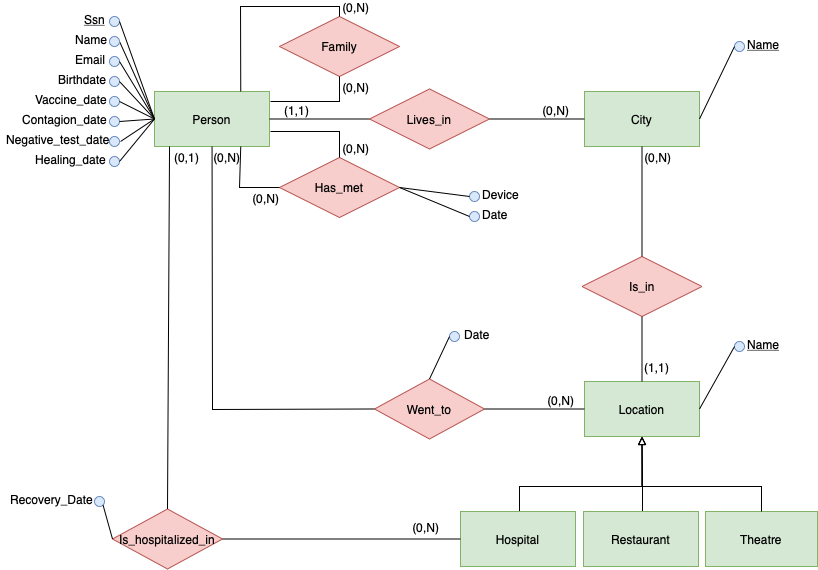
\includegraphics[scale=0.6]{er_diagram.png} % ER diagram
    }
    \caption*{The diagram represents the first phase of the database design.} % Caption
\end{figure}

\noindent % Removes indentation after the image
The diagram per se should be already auto-explicative. However, for better 
clarity, a more detailed description of each entity along with reasons of why 
such elements should be present in the database is provided:

\begin{itemize}
    \item \texttt{Person}: it contains information that allows the system to
        keep track of the users and perform analytics on them.  
    \item \texttt{City}: it contains information regarding cities that are
        present in the system. It can be useful to check where a person lives
        or a location resides in order to aggregate useful data.
    \item \texttt{Location}: it contains information regarding buildings that 
        are present in the system and where people can be tracked explicitly. 
        In the implementation, the various specializations of the 
        \emph{Location} "relation" were merged into the parent with the help
        of an attribute named \texttt{type}.
    \item \texttt{Hospital}: it is a specialization of the location entity. 
        Given the current emergency, hospitals can offer hospitalization rooms 
        for patients with \emph{COVID-19} but can also be visited like other 
        locations. 
    \item \texttt{Restaurant}: it is a specialization of the location entity. 
    \item \texttt{Theater}: it is a specialization of the location entity.  
\end{itemize}

\subsection{Dataset description}

We represented a population of 800 people in the USA, considering xxx locations
between xx cities; data is recorded from February 2020. \todo{fill with db data} \\ 
We used three types of nodes: Person, Location and City. 
People are characterized by their name (composed by name and surname), 
birthdate, city, email, social security number, vaccine date, date of the last 
contagion, date of the last negative test and healing date. \\
Locations have a name and a type (restaurant, theater, hospital); 
type is used so that the dataset can be easily expanded with new types of 
locations. \\
Possible relationships are: 
\begin{itemize}
    \item \texttt{WENT\char`_TO} to track people who visited a location at a 
        certain time;
	\item \texttt{IN\char`_FAMILY} for family relationships;
	\item \texttt{IS\char`_IN} between locations and cities;
	\item \texttt{LIVES\char`_IN} to link people to the city they live in;
    \item \texttt{HAS\char`_MET} to indicate contacts between people using 
        tracing app or devices;
    \item \texttt{IS\char`_HOSPITALIZED\char`_IN} to indicate people who 
        are/were hospitalized for covid reasons.
\end{itemize}

\noindent % Removes indentation after list
The complete script used for the creation of the database, togheter with a 
database dump will be provided alongside this document.

\subsection{Queries}

Only the most significative queries are shown in this document. \\
All the implemented queries will be provided alongside this document.

\subsubsection{Average age}

\begin{tcolorbox}[fontupper=\scriptsize]
    \begin{verbatim}
WITH    apoc.date.convert(timestamp(), "ms", "d") AS now
MATCH   (pc:Person)
WHERE   pc.contagion_date IS NOT NULL AND
        NOT EXISTS((pc)-[:IS_HOSPITALIZED_IN]->(:Location {type:"Hospital"}))
WITH    apoc.date.parse(toString(pc.birthdate), "d", "yyyy-MM-dd") AS pc_birth,
        now
MATCH   (ph:Person)
WHERE   EXISTS((ph)-[:IS_HOSPITALIZED_IN]->(:Location {type:"Hospital"}))
WITH    apoc.date.parse(toString(ph.birthdate), "d", "yyyy-MM-dd") AS ph_birth,
        now, pc_birth

RETURN  avg((now-pc_birth)/365) AS avg_age_nothospitalized, 
        avg((now-ph_birth)/365) AS avg_age_hospitalized;
    \end{verbatim}
\end{tcolorbox}

\noindent % Removes indentation after box
Returns the average age for infected (but not hospitalized) and for infected 
and hospitalized people inside the database.

\subsubsection{Cities}

\begin{tcolorbox}[fontupper=\scriptsize]
    \begin{verbatim}
MATCH (cities:City)<-[LIVES_IN]-(person:Person) 
WHERE person.contagion_date >= $date1 AND person.contagion_date <= $date2
WITH cities, count(*) AS infected
ORDER BY infected DESC
RETURN cities.name, infected
    \end{verbatim}
\end{tcolorbox}

\noindent % Removes indentation after box
Return cities and the number of infected people in a given span of time. Results are sorted by the number of infected people. 
Takes the following parameters: 
\begin{itemize}
    \item \texttt{\$date1} \emph{(datetime)}: starting date;
    \item \texttt{\$date2} \emph{(datetime)}: ending date.
\end{itemize}

\subsubsection{Devices}

\begin{tcolorbox}[fontupper=\scriptsize]
    \begin{verbatim}
MATCH   (p1:Person)-[met:HAS_MET]->(p2:Person)
WITH    apoc.date.parse(toString(p1.contagion_date), "ms", "yyyy-MM-dd") 
            AS p1_contagion_date,
        apoc.date.parse(toString(p1.healing_date), "ms", "yyyy-MM-dd") 
            AS p1_healing_date,
        apoc.date.parse(toString(p2.contagion_date), "ms", "yyyy-MM-dd") 
            AS p2_contagion_date,
        met
WHERE   p1_contagion_date IS NOT NULL AND
        (p2_contagion_date IS NULL OR p2_contagion_date > p1_contagion_date)
WITH    apoc.date.add(p1_contagion_date, "ms", -14, "d") AS contagion_l,
        met, p1_healing_date
WHERE   met.date.EpochMillis >= contagion_l AND
        (p1_healing_date IS NULL OR met.date.EpochMillis < p1_healing_date)
RETURN  met.device, count(DISTINCT met) AS infected_contacts;
    \end{verbatim}
\end{tcolorbox}

\noindent % Removes indentation after box
Returns the number of contacts registered for each type of device.

\subsubsection{Infected}
\begin{tcolorbox}[fontupper=\scriptsize]
    \begin{verbatim}
MATCH   (p:Person)
WHERE   p.contagion_date IS NOT NULL AND
        p.contagion_date >= $date1 AND p.contagion_date <= $date2
RETURN  count(p);
    \end{verbatim}
\end{tcolorbox}

\noindent % Removes indentation after box
Returns the number of infected people over a given span of time. \\
Takes the following parameters: 
\begin{itemize}
    \item \texttt{\$date1} \emph{(date)}: starting date;
    \item \texttt{\$date2} \emph{(date)}: ending date.
\end{itemize}

\subsubsection{Locations}
\begin{tcolorbox}[fontupper=\scriptsize]
    \begin{verbatim}
MATCH (places:Location)<-[r:WENT_TO]-(person:Person)
WHERE $date1 <= r.date AND r.date <= $date2
WITH places, count(*) AS infected
ORDER BY infected DESC
RETURN places.name, infected
    \end{verbatim}
\end{tcolorbox}
\noindent % Removes indentation after box
Returns locations and the corresponding number of people who went there and possibly got infected in a certain span of time. Results are sorted according to the number of visits. \\
Takes the following parameters: 
\begin{itemize}
    \item \texttt{\$date1} \emph{(datetime)}: starting date;
    \item \texttt{\$date2} \emph{(datetime)}: ending date.
\end{itemize}

\subsubsection{Notifications}

\begin{tcolorbox}[fontupper=\scriptsize]
    \begin{verbatim}
MATCH   (p:Person {ssn:$ssn})
WHERE   p.contagion_date IS NOT NULL
CALL {
        WITH    p
        CALL    apoc.path.expandConfig(p, {
                        relationshipFilter: "FAMILY>",
                        minLevel: 1,
                        maxLevel: -1,
                        labelFilter: "+Person",
                        uniqueness:"NODE_GLOBAL",
                        bfs:true
        }) YIELD path AS path
        UNWIND tail(nodes(path)) AS x
        WITH DISTINCT x AS contact
        RETURN  contact, "family" AS tracing, null AS time

        UNION

        WITH    p
        MATCH   (p)-[met:HAS_MET]->(pc:Person)
        WITH    apoc.date.parse(toString(p.contagion_date), "ms", "yyyy-MM-dd") 
                    AS contagion_date,
                apoc.date.parse(toString(p.healing_date), "ms", "yyyy-MM-dd") 
                    AS healing_date,
                pc, met
        WITH    apoc.date.add(contagion_date, "ms", -14, "d") AS contagion_l,
                pc, met, healing_date
        WHERE   (met.date.EpochMillis >= contagion_l) AND 
                (met.date.EpochMillis < healing_date OR healing_date IS NULL)
        RETURN  pc AS contact, met.device AS tracing, met.date AS time

        UNION

        WITH    p
        MATCH   (p)-[go1:WENT_TO]->(loc:Location)<-[go2:WENT_TO]-(pl:Person)
        WITH    apoc.date.parse(toString(p.contagion_date), "ms", "yyyy-MM-dd") 
                    AS contagion_date,
                apoc.date.parse(toString(p.healing_date), "ms", "yyyy-MM-dd") 
                    AS healing_date,
                pl, go1, go2, loc
        WITH    apoc.date.add(contagion_date, "ms", -14, "d") AS contagion_l,
                apoc.date.add(go1.date.EpochMillis, "ms", -2, "h") AS go1_l,
                apoc.date.add(go1.date.EpochMillis, "ms", 2, "h") AS go1_u,
                pl, go1, go2, loc, healing_date
        WHERE   go2.date.EpochMillis >= go1_l AND 
                go2.date.EpochMillis <= go1_u AND
                go1.date.EpochMillis >= contagion_l AND 
                (go1.date.EpochMillis < healing_date OR healing_date IS NULL)
        RETURN  pl AS contact, loc.name AS tracing, go1.date AS time
}
RETURN DISTINCT contact, collect({tracing:tracing, time:time}) AS info;
    \end{verbatim}
\end{tcolorbox}

\noindent % Removes indentation after box
Returns a list of people that a specific infected person (given their 
\emph{social security number}) may has been in contact with, considering 
family relationships, contacts from device tracking and inferred contacts from
explicit data collection in specific locations. \\
For each contact we offer complete information on the person that came in 
contact with the infected and, when possible, place/device information and 
time of the contact. \\
Takes the following parameters: 
\begin{itemize}
    \item \texttt{\$ssn} \emph{(string)}: social security number of the 
        infected person.
\end{itemize}

\subsubsection{Vaccinated}

\begin{tcolorbox}[fontupper=\scriptsize]
    \begin{verbatim}
MATCH (p:Person)
WHERE p.contagion_date >= p.vaccine_date
WITH count(*) AS vaccinated
MATCH (p1: Person)
WHERE p1.contagion_date IS NOT NULL
RETURN (toFloat(vaccinated)/count(*))*100
    \end{verbatim}
\end{tcolorbox}

\noindent % Removes indentation after box
Returns the percentage of vaccinated infected people over the total 
number of infected (considering also the non-vaccinated).


\subsection{Commands}

Only the most significative commands are shown in this document. \\
All the implemented commands will be provided alongside this document.

\subsubsection{Contact}

\begin{tcolorbox}[fontupper=\scriptsize]
    \begin{verbatim}
MATCH   (a:Person {ssn:$ssn1}), (b:Person {ssn1:$ssn2})
CREATE  (a)-[r:HAS_MET {date:$date, device:$device}]->(b), 
        (b)-[r:HAS_MET {date:$date, device:$device}]->(a);
    \end{verbatim}
\end{tcolorbox}

\noindent % Removes indentation after box
Registration of a contact via device.
Takes the following parameters: 
\begin{itemize}
    \item \texttt{\$ssn1} \emph{(string)}: social security number of the 
        first person;
    \item \texttt{\$ssn2} \emph{(string)}: social security number of the
        second person;
    \item \texttt{\$date} \emph{(datetime)}: date and time of the contact;
    \item \texttt{\$device} \emph{(string)}: type of device that detected a 
        contact.
\end{itemize}

\subsubsection{Negative test}

\begin{tcolorbox}[fontupper=\scriptsize]
    \begin{verbatim}
MATCH (p {ssn: $ssn})
WITH p,
    CASE 
        WHEN p.healing_date IS NULL AND p.contagion_date IS NOT NULL 
        THEN $test_date
        ELSE p.healing_date
    END 
    AS healing
SET p.negative_test_date = $test_date, p.healing_date = healing
    \end{verbatim}
\end{tcolorbox}

\noindent % Removes indentation after box
Registration of a negative COVID test. It updates the date of the last negative test of the person with the given SSN; if the person was infected, the healing date is updated with the date of the test, otherwise it is not changed.
Takes the following parameters: 
\begin{itemize}
    \item \texttt{\$ssn} \emph{(string)}: social security number;
    \item \texttt{\$test\_date} \emph{(date)}: date of the negative test.

\end{itemize}

\subsubsection{Positive test}
\begin{tcolorbox}[fontupper=\scriptsize]
    \begin{verbatim}
MATCH (p {ssn: $ssn})
WITH p,
    CASE 
        WHEN p.contagion_date IS NOT NULL THEN p.contagion_date
        ELSE $test_date
    END 
    AS infection
SET p.contagion_date = infection
    \end{verbatim}
\end{tcolorbox}

\noindent % Removes indentation after box
Registration of a positive COVID test. The contagion date is set equal to the test date, considering that if a person got covid, he/she cannot get it again (in this case the contagion date is not updated).
Takes the following parameters: 
\begin{itemize}
    \item \texttt{\$ssn} \emph{(string)}: social security number;
    \item \texttt{\$test\_date} \emph{(date)}: date of the positive test.
\end{itemize}

\clearpage

% APPLICATION
\section{Application}

\subsection{Description}

\blindtext

\subsection{User Guide}

\blindtext

\clearpage

% REFERENCES AND SOURCES
\section{References and sources}

\blindtext

\clearpage

\end{document}